%%%%%%%%%%%%%%%%%%%%%%%%%%%%%%%%%%%%%%%%%
% University/School Laboratory Report
% LaTeX Template
% Version 3.1 (25/3/14)
%
% This template has been downloaded from:
% http://www.LaTeXTemplates.com
%
% Original author:
% Linux and Unix Users Group at Virginia Tech Wiki 
% (https://vtluug.org/wiki/Example_LaTeX_chem_lab_report)
%
% License:
% CC BY-NC-SA 3.0 (http://creativecommons.org/licenses/by-nc-sa/3.0/)
%
%%%%%%%%%%%%%%%%%%%%%%%%%%%%%%%%%%%%%%%%%

%----------------------------------------------------------------------------------------
%	PACKAGES AND DOCUMENT CONFIGURATIONS
%----------------------------------------------------------------------------------------

\documentclass[12pt,a4paper]{article}

%\usepackage[version=3]{mhchem} % Package for chemical equation typesetting
%\usepackage{siunitx} % Provides the \SI{}{} and \si{} command for typesetting SI units
\usepackage{graphicx} % Required for the inclusion of images
\usepackage{geometry}
%\usepackage{natbib} % Required to change bibliography style to APA
%\usepackage{amsmath} % Required for some math elements 
%\usepackage{enumerate}
\usepackage{indentfirst}
%\setlength\parindent{24pt}


%\renewcommand{\labelenumi}{\alph{enumi}.} % Make numbering in the enumerate environment by letter rather than number (e.g. section 6)

%\usepackage{times} % Uncomment to use the Times New Roman font

%----------------------------------------------------------------------------------------
%	DOCUMENT INFORMATION
%----------------------------------------------------------------------------------------

\title{Improvements for Congestion Control Algorithms in Large-Scale Datacenter Network \\ Algorithm Adjustment for DCQCN \\ undergraduate dissertation} % Title

\author{Yuchen \textsc{Yang}} % Author name

\date{\today} % Date for the report

\begin{document}

\maketitle % Insert the title, author and date

\begin{center}
\begin{tabular}{l}
141242048 \\
Kuang Yaming Honors School, Nanjing University \\
ranchyang96@gmail.com \\
Instructor: Professor Chen Tian
\end{tabular}
\end{center}


\begin{abstract}
	Modern datacenters are experiencing a fierce increase in scale and traffic bandwidth.
	Remote Direct Memory Access (RDMA) permits high-throughput, low-latency networking,
	which is especially useful in such a large-scale scenario.
	The most primitive method (like TCP/IP stack) for congestion control is to drop packets when the receiver buffer is full.
	Later we have Piriority-based Flow Control (PFC) to generate congestion information in ACKs.
	Before this paper, we have Datacenter Quantized Congestion Notification (DCQCN) which uses the state-of-the-art scheme for congestion control.
	However, we may find DCQCN incapable of some large-scale traffic scenarios.
	In this paper, we analyze the drawbacks of DCQCN.
	At the same time, we present our improvements to DCQCN and name it DCQCN+.
	Improvements mainly focus on the adaptive increasing step and intervals.
	We have implemented them on testbed testbeds and NS3 simulation.
	Our method has the 10 times smaller latency than DCQCN under large-scale conditions (400+:1 incast) and 4 times larger flow capability than DCQCN.
	While in small incast cases, we have similar performance with DCQCN.
	This paper additionally focuses on my own work, about the testbed implementation and configurations of the method.
	It actually includes many detailed methods used for execution of experiments and detailed information about testbed experiment results.
\end{abstract}


\section{Introduction}

Modern datacenters are experiencing a fierce increase in both scale and bandwidth.
As we know, datacenters need small RTTs (some may be even tens of microseconds),
ability to handle burst flows for incasts and support the equality and balancing for concurrent flows.
Traditional TCP/IP stack surely can't do the job.
When encountering a large number of concurrent flows, TCP may choose to drop packets when the receiver buffer is full.
That's not tolerable for sure in datacenters since datacenters require lossless network to ensure the security and accuracy in large-scale traffic.
Then the first idea coming is to find a way to predict the congestion of the receiver end.
We hope to let the sender get some information about the receiver.

Then we get Explicit Congestion Notification (ECN) at the beginning.
This method uses a mark in the IP header from the ACK.
If the receiver dropped a packet, it echoes the congestion indication to the sender, so that the sender can reduce its sending rate.
Such ECN flags indicate the existance of congestion of receiver side after congestions have already happened.
ECN somehow relieves the congestion and make the receiver side drop fewer packets, but this still can't be lossless.

Later Quantized Congestion Notification (QCN) is developed.
QCN enables the switch to control the packet sending rate of an Ethernet source whose packets are traversing the switch.
This maintains a stable queue occupancy and is easy to be implemented on hardwares.
QCN is also applicable for multiple flows in a same port.

Priority-based Flow Control (PFC) applies the PAUSE frame to make things better.
PAUSE is used by the receiver to send feedback on the sender about the buffer space.
PFC actually divide services into 8 classes to make the feedback information more accurate.
Since the PAUSE frame carries more information, sender can know the exact remaining space in receiver buffer.
Thus the reaction on sending rate can be more accurate.
However this method can't be specific on flows but only on ports, which is usually combined with ECN to make it work better.

Before this paper, we have Datacenter QCN (DCQCN) which handles congestion better and is the essence of our work.
DCQCN is the application of QCN on datacenters, which divides the overall algorithms into three parts.
A brandnew concept mentioned here is Congestion Notification Packet (CNP), which functions similarly as PAUSE frame in PFC but carries more informations.
CNP packets are actually sent by NP which is the receiver end.
Each time when a packet with ECN mark is got and there are no CNP packets sent during the last interval time, a CNP is sent to notify the
sender.
Here the interval time mentioned is usually a interval time set up in advance by hardware to make sure that there won't be a CNP burst on
RP side.
This interval is also greatly limited by hardware ability.
Detailed information is also be mentioned in later sections.

In the end I briefly introduce the most important points about our new method DCQCN+.
DCQCN+ deploys dynamic rate control mechanisms to adapt incast of different scales instead of the fixed rate control for DCQCN.
What I'm in charge of is the testbed configuration and experiments.

The paper is organized as follows.
In Section 2 we introduce the background of the project.
In Section 3 we present limitations of DCQCN and necessity for improvements.
In Section 4 we show possible improvements for DCQCN.
In Section 5 I display detailed methods used for testbed experiments.
In Section 6 we show the results of experiments.
In Section 7 and 8, there are some discussions and future work.

\section{Background}
\subsection{Mellanox switch and ConnectX-4}
In the testbed experiments, we are using Mellanox SN2700 switch and ConnectX-4 Network Interface Cards.
Mellanox SN2700 carries a huge throughput of 6.4Tb/s, 32 ports at 100GbE.
The port speed can actually vary from 10Gb/s, 25Gb/s, 40Gb/s and 100Gb/s.
All 32 ports are connected to 16 machines inside our testbed with 2 each, but only 9 ports on 9 separate machines are used inside our
testbed experiments.

ConnectX-4 EN adapter can support 100Gbps Ethernet Connectivity.
Its Virtual Protocol Interconnect also supports EDR 100Gbps InfiniBand traffic.
We have ConnectX-4 adapters on all machines in our testbed.
Additionally we have tested the ability of ConnectX-5 adapters on a new testbed about the Congestion Notification Packet generation
ability.
This will described later.

\subsection{Remote Direct Memory Access}
Remote Direct Memory Access almost satisfy all the demands for datacenter networks.
It permits high throughput and low latency.
Similar to Direct Memory Access, RDMA actually allows user-space applications to directly read or write without the operation from
any operating systems.
Such network feature omits the possible copies inside systems thus performs better inside datacenters.

\subsection{Priority-based Flow Control}
Priority-based Flow Control ensures the lossless feature for RDMA.
No buffer packet overflow is a must for datacenter networks.

However, PFC actually does nothing to make the latency low.
When the receiver buffer is almost full, the packets inside the buffer queue up for a long time which makes the queueing latency
extremely high.
Such unfairness and high latency are fatal to datacenters and we hope to make up the drawbacks.

\subsection{Explicit Congestion Notification}
Explicit Congestion Notification is designed to indicate congestion to the sender.
An ECN-aware router may set a mark in the IP header instead of dropping a packet in order to signal impending congestion.
The receiver of the packet echoes the congestion indication to the sender,
which reduces its transmission rate as if it detected a dropped packet.

\subsection{DCQCN}
Datacenter Quantized Congestion Notification is explained in detail by \cite{dcqcn}.
Here I wil generally describe the mechanisms used in DCQCN.

Three parts of algorithms are developed.
The parts are Congestion Point (CP), Reaction Point (RP) and Notification Point (NP),
which are switches, senders and receivers respectively.
Both the switch and end points participate in to make things right.

For NP, i.e. receivers, they need to generate and send CNP when a packet with ECN mark and there is no CNP sent during the last interval.
CNPs are generated by receivers, indicating the remaining size of the receiving buffer.

For CP, a function of ECN marking probability P is related with Egress Queueing size S:

for $0<S<K_{min}$, $P = 0$

for $K_{min}<S<K_{max}$, $P = (S - K_{min})/(K_{max} - K_{min})*P_{max}$

for $S>K_{max}$, $P = 1$

which is shown in Figure ~\ref{fig:ECNMarking}.

\begin{figure}[h]
	\begin{center}
		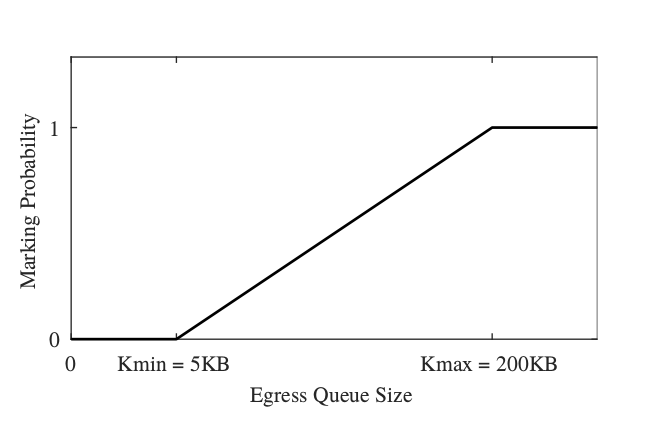
\includegraphics[width=3in]{ECNMarking}
		\caption{ECN Marking Probability for CP in DCQCN}
		\label{fig:ECNMarking}
	\end{center}
\end{figure}

Such marking probability is a brandnew idea from QCN.
Previously marking ECN or not is a fixed thing without possibility.
Such 0/1 resolution for ECN is not proper because that may cause the late reaction from sender.

\section{Problems of DCQCN}
The major problem for DCQCN is the failure of dealing with large-scale incast traffic.
Both in simulation and testbed experiments show that the switch buffer queue length remains high after a large burst at the beginning.

In testbed experiments, we actually find that when the flow number is under 400, the queue length will go down after 2 or 3 seconds.
Here the flows are continuous InfiniBand traffic lasting for about 80 seconds and they are started at approximately the same time.
There could be some turbulance of starting times but within 1 second.
This means that when the flow number is not large, convergence should be reached within 2 seconds.

However, when we start over 400 flows, the high queue length lasts till the end of all flows.
Convergence fails to be reached when the flow number gets really large.

Nowadays the tendency is that scale of datacenters go larger and larger which gives much pressure on datacenter networks.
Such a long queue length surely lead to high network latency or unfairness.
Thus the demand of datacenter network is not met.

In simulation results, we find even worse convergence effect.
Here from Figure ~\ref{fig:DCQCNfail}, we can see that 160 flows fail to be converged under 10Gbps links and 80 flows fail to 
be converged under 40Gbps links.
All the parameters used here are default parameters on Mellanox official forum, \cite{MellanoxOfficial}.

\begin{figure}[h]
	\begin{center}
		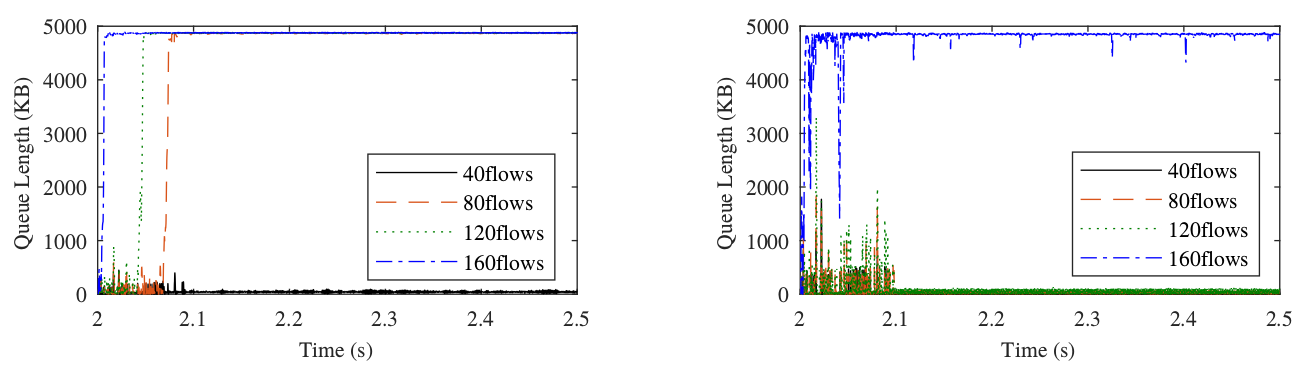
\includegraphics[width=6in]{DCQCNfail}
		\caption{DCQCN fails to converge}
		\label{fig:DCQCNfail}
	\end{center}
\end{figure}

\section{Improvements for DCQCN}

The key factor of DCQCN's failure is DCQCN's increase step, recovery speed and CNP supplies.
These information used are out of date for the growing scalability for data centers.
Those fixed increase steps, recovery speed and CNP intervals are not adaptive for large-scale traffic.
What we do is to find factors which actually influence the congestion and can predict the congestion level better.

Our work, DCQCN+ uses dynamic parameters to better analyze the congestion and therefore relieve it.
DCQCN never cares about the incast scale and thus uses fixed parameters to do the job.
That surely won't work for large-scale incast since the reaction and adjustments of sending rate are not very accurate.

DCQCN+ designs to use the CNP period carried in CNPs and the flow rate to reflect the condition of the incast scale.
There are some remaining available CNP fields to carry the period information of CNP.
Also, since larger flows are more probable to be marked with ECN, its possibility to trigger a CNP is larger.
Thus all congested flows can get similar rates and be balanced.

To be more specific, improvements are discussed from three points (Congestion Point, Notification Point and Reaction Point).

\subsection{Congestion Point}

This part remains almost the same.
What we can do at Congestion Point is really limited since CP is responsible for ECN marking.
The probability for ECN marks are very resonable so we leave this part the same.

We also need to mention here that PFC is still enabled to ensure lossless feature of datacenters.
Although our method can make sure that convergence can be reached in most cases, we can't ensure lossless feature at the starting burst
if PFC is disabled.

\subsection{Notification Point}

Receivers are in charge of generating CNPs.
This is the most important part of the algorithm.

At NP, two factors decide the CNP interval, the hardware ability of generating CNP and the demand for CNP at Reaction Point.
We hope to supply enough CNPs with shorter intervals for RP to properly adjust the sending rate.
At the same time we don't want to cause other problems like CNP burst or CNP congestion if we set the interval which is too short.
Such problems may cause unnecessary bandwidth cost.
The ability of hardware may incluence the minimal interval and demands for CNPs decide the maximal interval.
We prefer the maximal interval to relieve the possibility of bandwidth cost.

Once the flow rate collects enough information to decide the incast scale, the CNP interval should be decided.

\subsection{Reaction Point}

Here we first show the original DCQCN RP algorithm pseudocode in Figure ~\ref{fig:RPalg}.

We make some changes on the updates of parameters.

The reaction when receiving CNP is similar:
\[R_T=R_C\]
\[R_C=R_C(1-\alpha /2)\]
\[\alpha = (1-g)\alpha + g\]

Here $\alpha$ is a reduction factor, actually indicates the congestion level at the CP.
$R_C$ denotes current rate and $R_T$ denotes target rate.
$g$ is a parameter to estimate the congestion level.

Instead of DCQCN's fixed rate increase timer $K=55\mu s$, we make it flexible:
\[K=\lambda max(\tau, \frac{MTU}{R_C})\]
where $MTU$ denotes Maximal Transmit Unit and $\tau$ denotes CNP interval.

Here we remove the byte counter and add the rate increase counter.
When the rate increase counter times out, the state S increses 1.

The fast recovery scheme remains the same when $S$ is less than the threshold $F = 5$:
\[R_C=\frac{R_C+R_T}{2}\]

When $F<S<4F$,
\[R_T=R_T+ min(\frac{1}{10}R_C,\frac{1}{100}R_l)\]
\[R_C=\frac{R_C+R_T}{2}\]
where $R_l$ is a ratio used to bound the increase step for small incast cases.

When $F>4F$, Hyper Increase is applied,
\[R_T=R_T+min(R_C, \frac{S-4F}{100}R_l)\]
\[R_C=\frac{R_C+R_T}{2}\]

Additionally, when $\alpha$ timer runs out,
\[\alpha=(1-g)\alpha\]

We can see a lot of changes to make the algorithm better.
Such dynamic adjustments of parameters greatly improve the buffer estimation in advance and drain the congestion fast
to maintain the buffer queue length low.

\section{Implementation}

We set up the testbed of testing for DCQCN+ on Mellanox SN2700 switch and 9 Ubuntu servers with ConnectX-4 adapter cards.
Mellanox SN2700 provides the most predictable, highest density 100GbE switching platform for the growing demands of today's data centers,
which satisfies our experiment environment for over 400 flows at a time.
ConnectX-4 dual-port adapter cards with Virtual Protocol Interconnect (VPI) support 100Gb/s InfiniBand and 100Gb/s Ethernet connectivity.
All the features including RoCEv2, PFC and ECN are supported on Mellanox SN2700 and ConnectX-4 adapter card.

To generate enough number of flows for our experiment, the topology is shown in Figure ~\ref{fig:topology}.

\begin{figure}[h]
	\begin{center}
		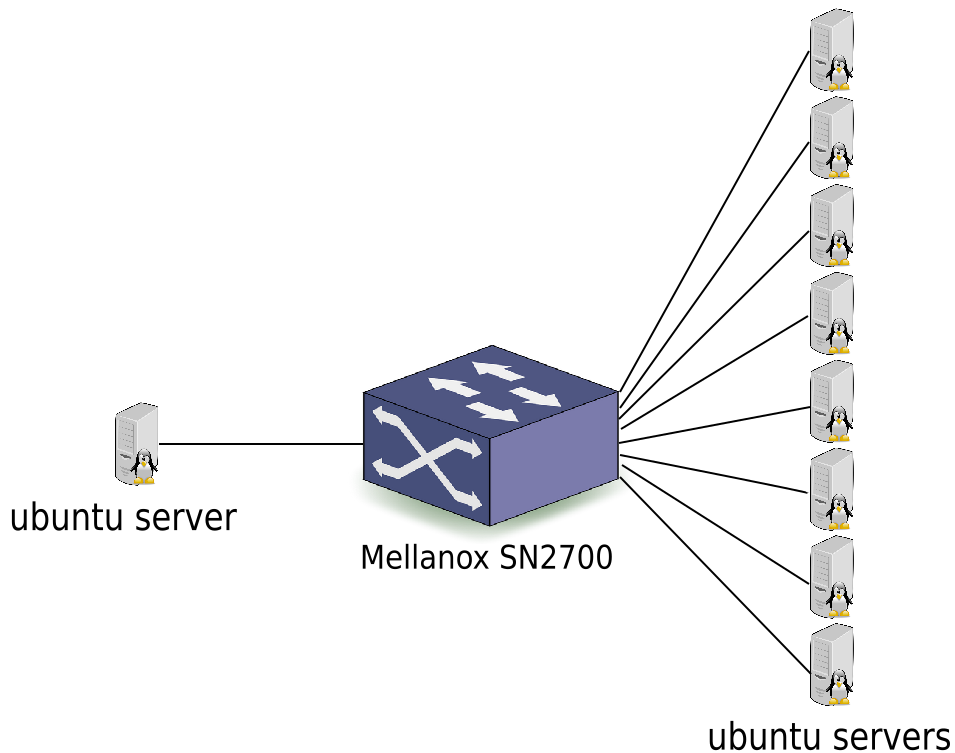
\includegraphics[width=3in]{topology}
		\caption{Topology for multi-flow tests}
		\label{fig:topology}
	\end{center}
\end{figure}

To be clear, we regard the server on the left (which is the receiver) as S0 and the servers on the right (which are senders) as S1 to S8.
All the servers are configured into the same virtual local area network (VLAN) so that we can construct an incast traffic inside the network.

\subsection{Switch Configuration}

Mellanox 2700N has provided a lot of interfaces for users. Among them, we need to configure VLAN, PFC, ECN and buffer size to make things work.

\subsubsection{VLAN}
The whole expetiment environment should be separated from outside traffic including SSH connection and SFTP file transmission.
VLAN is thus needed to create a separate topology.

Switch need to enable the VLAN feature and include all machines in the same VLAN session.
This includes some work on distinguishing ports.

\subsubsection{PFC}
PFC is needed because what we want is a lossless network which is a must for data center networks.
PFC makes receiver to send PAUSE frame to sender where sending ratio is limited upon received PAUSE.
Default PFC configuration contains 8 priority classes and we only have 2 used here.
The mapping is mentioned in the following subsection about ECN.

\subsubsection{ECN}
ECN priority is configured to make CNP working well. Higher priority is needed for higher traffic class.
Inside our experiments, there are mostly two classes of traffic. RDMA traffic is in traffic class 3 and should be mapped to swith priority 3.
Other traffic like TCP is in traffic class 0 and should be mapped to switch priority 0.
The reason is that the traffic for setting up a flow shouldn't be blocked. If we don't set the priority difference, the flow setup traffic for a flow
is blocked when there are really a large number of flows. The flow setup period should use higher priority so that more flows can be created.
About this point, we explain it in later sections.
And the probability to make a ECN mark should be configured the same as mentioned in DCQCN--.

\subsubsection{Buffer}
About the buffer size, we don't need to be very specific. The maximal buffer size inside Mellanox 2700N switch is 5.1MB.
One important factor to be consider is the buffer usage during the experiment process.
When a lot of flows are created, there must be a burst of buffer at the beginning.
After a short period of reaction time, the buffer usage should go down because the senders are limited by switch based on flows.
In the results, what we are hoping to see is that the beginning of the buffer is large but after the short reaction time, the buffer is low.
Thus the buffer here is only to handle the burst at the beginning.

\subsubsection{Additional Configurations}
To make things clear, we need to cut unnecessary parts of traffic.

We obviously don't contain loops inside our topology so that the spanning tree protocol is removed from the switch.

The interface speed is set to 100Gbps when testing the hardware ability of generating CNP.
For other most experiments, interface speed is configured as 10Gbps (reason is explained in later sections).

\subsection{NiC Configuration}
At the very beginning, we need to install Mellanox OFED (driver for ConnectX-4) for every server.

After that, we have several steps (most corresponds with the upper switch configurations):
\begin{enumerate}
	\item Enable PFC and set up the priority.
	\item Enable ECN for both InfiniBand traffic and TCP traffic.
	\item Set CNP priority and DSCP priority.
	\item Set priority for RDMA traffic.
	\item Open sniffer for Tcpdump to capture InfiniBand packets.
\end{enumerate}

\subsection{Experiment Process}

The general idea is creating an incast and observe the congestion point.
To be more specific, we are generating flows from S1~S8 (tens of flows from each) and observe the bandwidth tendency, latency and buffer usage.

However before all of that, the first experiment is to test the CNP generation speed for ConnectX-4 and ConnectX-5. 

\subsection{Ability to Generate CNP}

All NiC has limited ability. For ConnectX-4 and ConnectX-5, we hope to figure out the exact ability of doing this so that we can adjust the DCQCN efficiently.

The topology is simple. Two servers are connected to the switch, one as sender and one as receiver.
For the receiver side, the interface speed is set to 10Gbps. The sender side has an interface speed of 100Gbps.
Thus the congestion surely exist and we use Tcpdump to capture the packets during a short period of time.

Among the packets captured inside the Pcap file, we filter the traffic with right direction and right IP addresses out.
According to the timestamps, we can know something about the ability of ConnectX-4 and ConnectX-5.

\subsection{Bandwidth Testing}

Now the topology is the one shown in Figure ~\ref{topology}.
We use the command ib\_send\_bw to start flows.


First let me introduce the key tools used here.
The mostly used library is Python Paramiko which provides secure connection for remote command execution and file transmission.
It's actually a Python implementation of SSHv2 protocol, providing functions of both server and client.
To be more specific, I contracted them down to four functions, one for connection checking, one for remote command execution and the other two for file
transmission between local and remote machines.
Everything here is using SSH protocol and thus my functions can be implemented by Python Paramiko.

Another point necessary to be mentioned here is multithreading. In the original version, the time for running is previously estimated.
Thus the execution time of the program is greatly increased or a command is run before its previous steps are finished.
Function ''join'' can correctly sequence all the steps in the program.

Bandwidth testing needs several steps:
\begin{enumerate}
	\item Refresh machine states.
	\item Time synchronization for all servers.
	\item Start Tcpdump simultaneously on S1~S8.
	\item Start ib\_send\_bw server on S0.
	\item Start ib\_send\_bw clients on S1~S8.
	\item Send Pcap files to local.
	\item Parse Pcap files.
	\item Use parsed results to draw bandwidth figure.
\end{enumerate}

The overall tests is done by scripts of many languages including Python, C, Bash, Awk and Gnuplot.

Let me describe the above steps one by one.

\subsubsection{State Refresh}

Because we start a large number of flows on each machine, the command of ib\_send\_bw may fail to complete correctly, leaving
some processes continuing during the stages. We need to refresh the states for mahcines.

To kill the processes running from the last experiment, we use the command ''pkill -f'' to kill processes with the label of ''ib\_send''.

\subsubsection{Time Synchronization}
We use Network Time Protocol (NTP) to synchronize the time for S0~S8.
The accuracy for NTP is about 0.01ms so that should work for servers on a rack.
Choosing a server inside the same rack, we set up an NTP server on it.

Then we use Python Paramiko to execute the NTP command on S0~S8 for time synchronization with the NTP server.

Here we need to claim a fact that the receiver side can't tolerate the amount of packets we need to actually generate a bandwidth figure.
Even an increased size of Tcpdump buffer can't hold the traffic of even 1 second which is obviously not enough to analyze the bandwidth tendency.
Thus we are running Tcpdump on each machine which can last for approximately 10 seconds.
With time synchronized, we can analyze packets on different machines with timestamps correct.

\subsubsection{Tcpdump Start}
Python Paramiko is still the tool used for remote command execution.

Different from normal Tcpdump, we need to specify several parameters here.
''-B 900000'' parameter is needed to increase the buffer size of Tcpdump.
''-s 60'' parameter is to capture only the first 60 bytes which contains just the packet headers.

It's hard to estimate the capturing time needed, but we can limit the packet counter of Tcpdump (which uses ''-c'').
Thus the file size is shrinked and it saves time for file transmission.

\subsubsection{ib\_send\_bw Server Client Starter}

This step contains concatenation work.
What we are doing is to accept parameters from the command line execution of the program.
This contains the concatenation of mark ''\&'' and other strings.
''\&'' is used for simultaneous command execution. Linux System usually has the ability to run over 1000 processes simultaneously.

Luckily string operations are easy for Python.
I'm actually recording the same parts of the commands and add loops with transformed string from numbers.

About the detailed information about the commands, we have several specific parameters set.
The parameter ''-R'' is for RDMA connection setup. However we find that using RDMA traffic for a flow start causes
the traffic congested with other already-started flows. Thus we may fail to start a lot of flows at the same time.
So in real experiments, we are not using the parameter.

The parameter ''-S 3'' means the priority class for RDMA traffic. This can also be set for ROCEv2 protocol.
We add it here just to be sure that the traffic class priority is working.

The parameter ''-x'' denotes the device ID we are using, which can be fetched through the command ''show\_gids''.
This displays the ROCE version we are using and the corresponding device ID and destination IP.
''show\_gids'' is only needed once for each machine so that it's not actaully included as part of the automation tool.

The parameter ''-d'' denotes the network devices used for the execution which is mlx5\_1 for our machines.

The parameter ''-D'' shows the lasting time of our experiment. It counts in seconds of the continuous sending procedure.
In our experiment it's usually 60 or 80 which shows almost a complete tendency of the bandwidth and flows.

The parameter ''-p'' is responsible for separating flows. In our experiment, we hope to create multiple flows from one machine.
The number could be tens and even reach 90 so we need to use port number to start different flows.
The actual implementation of port allocation is like this: 

We are taking parameters of machine number and flow number of each machine at the beginning of the overall scripts.
Assume that they are $m$ and $n$.
All port number for flows starts from 10011. There is a continuous range from 10011 to $10010+m\times n$ for port numbers.
The first machine takes the position of port number like 10011, $10011+m$, ..., $10011+m\times(n-1)$.
To be more general, the $i_{th}$ flow on the $j_{th}$ machine (where $i=1,2,...,n$ and $j=1,2,...,m$) has the port number of
$10010+i+m\times(j-1)$.
Thus all the port numbers don't collide with each other. This makes later steps easier to process.
Those are mentioned in later sections.

\subsubsection{File Transmission}
To be clear, we are running experiments on 9 machines.
Besides that, we have a middle machine with accounts to login, making the machines more secure.
And we have a local machine to process the results we get. We are using a local machine to do this because
we hope to keep the experiment machines clean and fewer new tools should be used there.

Thus the file transmission has two parts. First step would be sending Pcap files from experiment machines to the middle machine.
The second would transmitt the files from the middle machine to the local machine.

\subsubsection{Pcap Parsing}
This contains several steps. We can't make sure that this is the easiest way to process these packets but it works fine.
\begin{enumerate}
	\item Transform Pcap files to plain text.
	\item Filter the packets to get the traffic with the receiver we want.
	\item Divide the packets from all different flows in the same machine.
	\item Collect number of packets in every millisecond.
	\item Transform timestamps to relative time starting from the beginning of the flows.
	\item Add counts of zeros for those milliseconds which contains no packets.
\end{enumerate}

For step 1, I use the command of Tcpdump with the parameter of ''-r'' which means reading.
With option ''-rrrr'' and ''-nnq'' we transfer the Pcap file into plain text with 8 terms.
Among them we have the timestamp, source IP, source port, destination IP and destination port.
Thus we can approximately calculate the bandwidth from such informations.

For step 2, I use Awk to do the filtering. By limiting the receiver as the only host we regard as incast receiver, we get all the receiver IP (which is the
$6^{th}$ term of the plain text) out of all possible flow receivers.

For step 3, we can only devide all the flows on the same machine using the ports.
Tcp and InfiniBand has its unique port forwarding methods which would surely dismiss the ports I set for them in the ''ib\_send'' commands.
To separate all these flows, I write a C++ program to do the filtering work, collecting all the different port numbers and raise flags for new port numbers.
Each new port number starts a new file for collection, containing the packets of a single flow.
The file names are carefully calculated.
Suppose we have $m$ machines and each starts $n$ flows, then the numbering of the file names are similar to the one previously mentioned in port nubmering.
The only difference is that port numbers start from 10010 and the file names start from 85 (which is the machine index in our testbed).

For step 4, I specifically count the digits in every line (which contains a packet) of the plain text. Thus I can make sure which digits represent the condition
of the timestamps. 
Then I decide in plain text which exact digit decides the millisecond and which digit is the starting point of the timestamp.
To decide the amount of packets in one millisecond, we can find the ones with a sharing first 3 digits after the decimal point in the timestamp.
To do the filtering and counting work, we have an easy commandline tool which is ''cut''.
Using the option of ''-c'', we can have a count on the packet number with the same timetamp till millisecond digit.
We therefore print the timestamps and the packet numbers. (which has two columns and therefore can be drawn into a figure.

Step 5 and step 6 are relatively easy. 
Record the earliest packet occurs and do subtractions.
Then we need to add zeroes for those milliseconds which contains no packet to make the figure fluent and complete.

\subsubsection{Figure Plotting}

Here we use the tool of Gnuplot, which is a practical plotting tool under Linux systems.

Before we have figured out the timeline and packet count for each millisecond.
For most packets, they have the same size of 1KB which is fixed by the command ''ib\_send''.
Thus we can indicate the bandwidth through packet count of each millisecond.

\section{Results}

\section{Discussion}

\section{Conclusion and Future Work}


\bibliographystyle{apalike}

\bibliography{sample}

%----------------------------------------------------------------------------------------


\end{document}
